\documentclass[border=8pt]{standalone}
\usepackage{tikz}
\usepackage{xcolor}
\usetikzlibrary{positioning,arrows.meta,shapes.geometric,calc,matrix}

\definecolor{obsCol}{HTML}{E66101}
\definecolor{genCol}{HTML}{5E3C99}
\definecolor{qualCol}{HTML}{B2182B}
\definecolor{concCol}{HTML}{4DAF4A}
\definecolor{ambCol}{HTML}{6E6E6E}
\definecolor{genoCol}{HTML}{2166AC}
\definecolor{bgGray}{HTML}{F5F5F5}

% Figure 1, redrawn to match Algorithm 1: each leg is standardized to
% Cohen's d and classified on its own against d = 0.10; the family label is
% the OBS x MR combination. No pooling, no Cochran's Q, no quantitative
% branch. RCT outcomes enter only in Stage 2, after classification.
\begin{document}
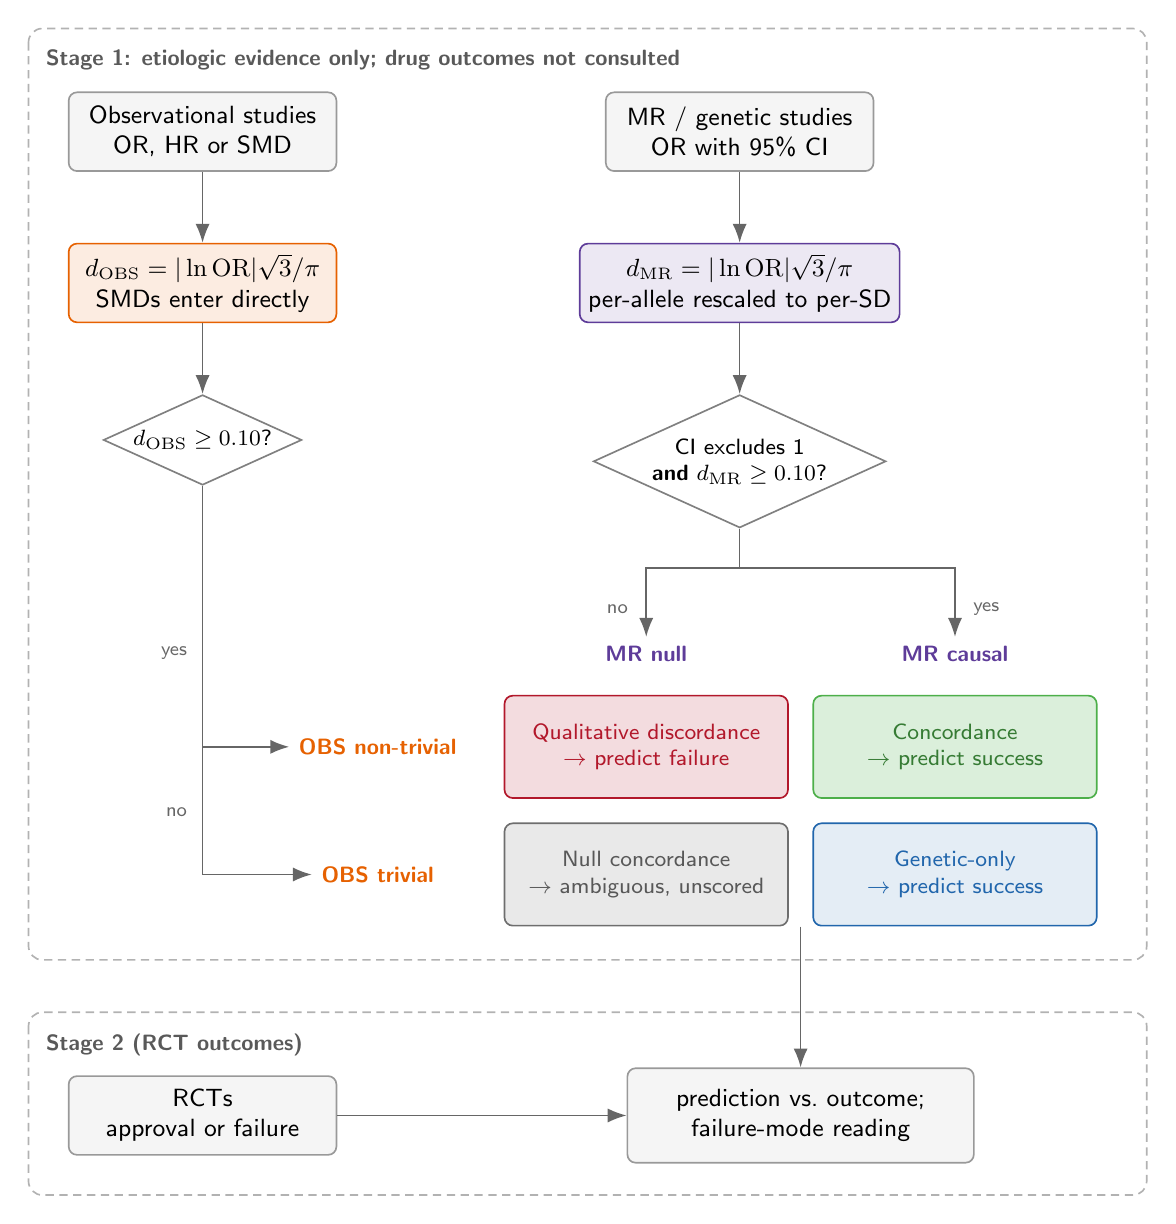
\begin{tikzpicture}[
    >={Latex[length=2.4mm,width=1.8mm]},
    font=\sffamily\small,
    node distance=9mm and 12mm,
    box/.style={rounded corners=3pt, draw, line width=0.6pt,
      minimum width=34mm, minimum height=10mm, align=center, inner sep=3pt},
    evidence/.style={box, fill=bgGray, draw=black!40},
    dec/.style={diamond, draw=black!50, fill=white, line width=0.6pt, aspect=2.2,
      inner sep=1pt, align=center, font=\sffamily\footnotesize},
    cell/.style={rounded corners=3pt, draw, line width=0.6pt, minimum width=36mm,
      minimum height=13mm, align=center, inner sep=3pt, font=\sffamily\footnotesize},
    arr/.style={->, line width=0.6pt, draw=black!60},
    lab/.style={font=\sffamily\scriptsize, text=black!60},
  ]

% Inputs
\node[evidence] (obs) {Observational studies\\OR, HR or SMD};
\node[evidence, right=34mm of obs] (mr) {MR / genetic studies\\OR with 95\% CI};

% Standardize
\node[box, fill=obsCol!12, draw=obsCol, below=of obs] (dobs)
  {$d_{\mathrm{OBS}} = |\ln \mathrm{OR}|\sqrt{3}/\pi$\\SMDs enter directly};
\node[box, fill=genCol!12, draw=genCol, below=of mr] (dmr)
  {$d_{\mathrm{MR}} = |\ln \mathrm{OR}|\sqrt{3}/\pi$\\per-allele rescaled to per-SD};

% Classify each leg on its own
\node[dec, below=of dobs] (cobs) {$d_{\mathrm{OBS}} \ge 0.10$?};
\node[dec, below=of dmr] (cmr) {CI excludes 1\\\textbf{and} $d_{\mathrm{MR}} \ge 0.10$?};

% 2 x 2 combination
\matrix[matrix of nodes, anchor=north west, at={($(cobs.south)+(8mm,-18mm)$)},
        column sep=3mm, row sep=3mm, nodes={anchor=center}] (grid) {
  \node[lab, minimum width=26mm, align=right] {}; &
  \node[lab, text=genCol, font=\sffamily\footnotesize\bfseries] (cnull) {MR null}; &
  \node[lab, text=genCol, font=\sffamily\footnotesize\bfseries] (ccaus) {MR causal}; \\
  \node[lab, text=obsCol, font=\sffamily\footnotesize\bfseries, align=right] (rnt) {OBS non-trivial}; &
  \node[cell, fill=qualCol!15, draw=qualCol, text=qualCol] (q) {Qualitative discordance\\$\to$ predict failure}; &
  \node[cell, fill=concCol!20, draw=concCol, text=concCol!70!black] (c) {Concordance\\$\to$ predict success}; \\
  \node[lab, text=obsCol, font=\sffamily\footnotesize\bfseries, align=right] (rtr) {OBS trivial}; &
  \node[cell, fill=ambCol!15, draw=ambCol, text=ambCol!80!black] (n) {Null concordance\\$\to$ ambiguous, unscored}; &
  \node[cell, fill=genoCol!12, draw=genoCol, text=genoCol] (g) {Genetic-only\\$\to$ predict success}; \\
};

% Arrows: inputs to d, d to decision, decisions to the grid axes
\draw[arr] (obs) -- (dobs);
\draw[arr] (mr) -- (dmr);
\draw[arr] (dobs) -- (cobs);
\draw[arr] (dmr) -- (cmr);
% OBS decision feeds the rows, MR decision feeds the columns
\coordinate (obsbus) at ($(grid.west)+(-9mm,0)$);
\draw[arr] (cobs.south) |- (rnt.west) node[lab, pos=0.32, anchor=east, xshift=-2pt] {yes};
\draw[arr] (cobs.south) |- (rtr.west) node[lab, pos=0.42, anchor=east, xshift=-2pt] {no};
\draw[arr] (cmr.south) -- ++(0,-5mm) -| node[lab, pos=0.8, anchor=east, xshift=-3pt] {no} (cnull.north);
\draw[arr] (cmr.south) -- ++(0,-5mm) -| node[lab, pos=0.8, anchor=west, xshift=3pt] {yes} (ccaus.north);

% Stage 1 bracket: everything above and including the grid
\draw[densely dashed, black!30, line width=0.6pt, rounded corners=5pt]
  ($(obs.north west)+(-5mm,8mm)$) rectangle ($(grid.south east)+(5mm,-3mm)$);
\node[anchor=north west, font=\sffamily\footnotesize\bfseries, text=black!65] at ($(obs.north west)+(-4mm,6.5mm)$)
  {Stage 1: etiologic evidence only; drug outcomes not consulted};


% Stage 2: its own bracket, the RCTs as an evidence input, one reading box
\coordinate (cellmid) at ($(n.south)!0.5!(g.south)$);
\node[box, fill=bgGray, draw=black!40, minimum width=44mm, minimum height=12mm] (read)
  at ($(cellmid)+(0,-24mm)$) {prediction vs.\ outcome;\\failure-mode reading};
\node[evidence] (rct) at (obs.south |- read) {RCTs\\approval or failure};
\draw[arr] (cellmid) -- (read.north);
\draw[arr] (rct.east) -- (read.west);
\draw[densely dashed, black!30, line width=0.6pt, rounded corners=5pt]
  ($(obs.west |- rct.north)+(-5mm,8mm)$) rectangle ($(grid.east |- read.south)+(5mm,-4mm)$);
\node[anchor=north west, font=\sffamily\footnotesize\bfseries, text=black!65]
  at ($(obs.west |- rct.north)+(-4mm,6.5mm)$) {Stage 2 (RCT outcomes)};

\end{tikzpicture}
\end{document}
